\documentclass[letterpaper,11pt]{article}

\usepackage{plg_ms}
\usepackage{lipsum}

\title{The Title Of The Paper}

\author[1]{Jane Doe \orcidlink {0000-0000-0000-0000}}
\author[1,2]{Paul L. Gribble \orcidlink {0000-0002-1368-032X}}
\affil[1]{Dept. Psychology, Western University, London, ON, Canada}
\affil[2]{Dept. Physiology \& Pharmacology, Schulich School of Medicine \& Dentistry, London, ON, Canada}

\date{}



\begin{document}

\maketitle
\thispagestyle{empty}

\textit{\small \today}

\vfill

\textbf{Correspondence}\\pgribble@uwo.ca\par
{\flushleft \textbf{Keywords}\\human; motor learning; motor cortex; proprioception; arm movement}\par

\newpage
\linenumbers

\begin{abstract}
\lipsum[1]
\end{abstract}

\newpage
\section*{Introduction}

\lipsum[2-4] The quick brown fox jumped over the lazy dog \citep{Codol_2023, Kistemaker2010-de}.

\section*{Results}

\lipsum[5-6] You can see some things in Figure~\ref{fig:methods}.

\begin{figure}[H]
\centering
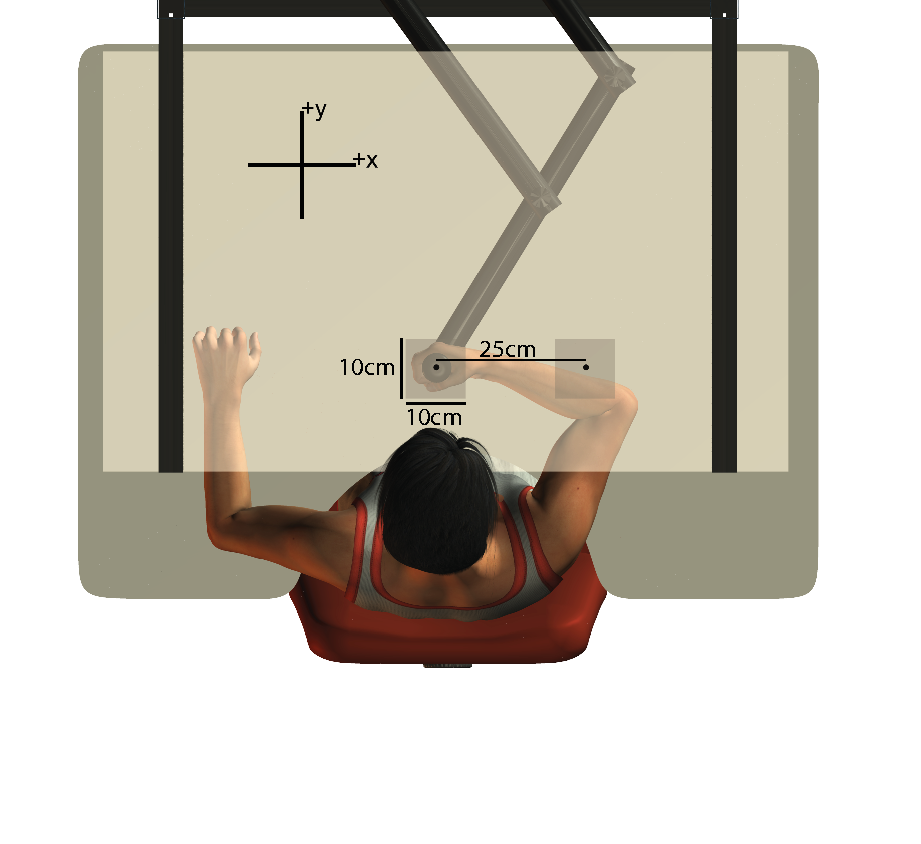
\includegraphics[width=0.75\linewidth]{figure1.pdf}
\caption{\textbf{A phrase about the figure}. \lipsum[7]}
\label{fig:methods}
\end{figure}

\lipsum[7-8]

\section*{Discussion}

\lipsum[9-11]


\newpage
\section*{Methods}

\subsection*{Participants}
\lipsum[12]

\subsection*{Experimental Sequence}
\lipsum[13-14]


\newpage
\nolinenumbers
\bibliography{refs}

\end{document}
